\documentclass[conference]{IEEEtran}
\usepackage{cite}
\usepackage{hyperref}
\usepackage{graphicx}
\usepackage{amsmath,amssymb,amsfonts,bm}
\usepackage{algorithmic}
\usepackage{textcomp}
\usepackage{xcolor}
\usepackage[caption=false,justification=centering]{subfig}

\newcommand*{\vertbar}{\rule[-1ex]{0.5pt}{1.5em}}
\newcommand*{\horzbar}{\rule[0.5ex]{1.5em}{0.5pt}}

\def\BibTeX{{\rm B\kern-.05em{\sc i\kern-.025em b}\kern-.08em
    T\kern-.1667em\lower.7ex\hbox{E}\kern-.125emX}}
\begin{document}

\title{Numerical Simulation of Self-Driven Particle Collective Motion}

\author{Reed Foster}

\maketitle

%\begin{abstract}
%\end{abstract}
%
%\begin{IEEEkeywords}
%\end{IEEEkeywords}

\section{Introduction}

Collective motion is an observable phenomenon ubiquitous to systems of self-driven particles.
It is most readily observed in living systems, such as murmurations of starlings, schooling of fish, and swarming of locusts.
It is even observed in non-living systems and microbes \cite{Vicsek}.
However, the qualitative behavior and pattern of motion observed by these different groups can vary widely.
In this work, my goal is to develop a model for collective motion that describes the equations of motion for self driven particles in a group that is generalizable to produce a variety of motion patterns.
The model draws heavily from the idea of zoning from \cite{Couzin}, in which each entity in a swarm categorizes its neighbors depending on how far they are from it.
It also incorporates a model for flexible leadership in which the role of leader shifts fluidly between entities as the structure of the swarm changes.

\section{Methods}

\subsection{Newton Equations and Neighbor Regions}

\begin{figure}[htbp]
    \centering
    \resizebox{0.9\columnwidth}{!}{\input{regions.pdf_tex}}
    \caption{Neighbor search regions}
    \label{fig:regions}
\end{figure}

The self-driven particles update their position and velocity using a method similar to that described in \cite{Couzin}.
As described in \cite{Couzin}, each entity tracks the velocity and position of neighbors within three different regions (Fig. \ref{fig:regions}), and uses that velocity and position data to update its own velocity vector.
Just as in the paper, my model uses the repulsion, orientation, and attraction zones/regions.
The type of effect (repelling, orienting/aligning, or attracting) a neighbor has on the entity depends on its position relative to the entity (both distance and direction relative to the entity's velocity vector).
However, in my model, there isn't a discrete transition of behavior between the different regions.
That is, an entity's perturbing force is always derived from its neighbors within all three regions (although the effects are weighted differently depending on the velocity and location of the neighbors).

The Newton equations for each entity $i$ are given by
\begin{IEEEeqnarray}{rCl}
    \dot{\mathbf{x}}_i(t) & = & \mathbf{v}_i(t) \\
    \dot{\mathbf{v}}_i(t) & = & \gamma_{V_{n_0}}\mathbf{V}_{n_i}(t) + \gamma_{cm_0}\mathbf{x}_{cm_i}(t) + \gamma_{\xi_0}\bm{F}_{\bm{\xi}_i}(t)
    \IEEEeqnarraynumspace
    \label{eqn:newton}
\end{IEEEeqnarray}

where $\mathbf{V}_{n_i}(t)$ and $\mathbf{x}_{cm_i}(t)$ are weighted averages of the velocities and displacements (relative to $i$) of the neighbors of $i$.
$\bm{F}_{\bm{\xi}_i}(t)$ is a smoothed random process defined by the differential equation:

\begin{equation}
    \dot{\bm{F}}_{\bm{\xi}_i}(t) = \tau_\xi\left(\bm{\xi}_i(t) - \bm{F}_{\bm{\xi}_i}(t)\right)
    \label{eqn:randomlowpass}
\end{equation}

where $\bm{\xi}_i(t)$ are $N$ i.i.d. Gaussian white noise processes.
By defining the forcing term $\bm{F}_{\bm{\xi}_i}(t)$ with such a differential equation, the random motion of the entities is driven by a low frequency signal, since equation \ref{eqn:randomlowpass} describes a lowpass filter.

\begin{figure}[htbp]
    \centering
    \subfloat[]{\resizebox{0.4\columnwidth}{!}{\input{position_conformity.pdf_tex}}}
    \par
    \subfloat[]{\resizebox{0.4\columnwidth}{!}{\input{velocity_conformity.pdf_tex}}}
    \par
    \subfloat[]{\resizebox{0.4\columnwidth}{!}{\input{repulsion.pdf_tex}}}
    \caption{Graphical depiction of how forcing terms in equation \ref{eqn:newton} are derived}
\end{figure}

\subsection{Leader Factor}

\begin{figure}[htbp]
    \centering
    \subfloat[High leader factor]{
        \resizebox{0.20\columnwidth}{!}{\input{high_leader_factor.pdf_tex}}
        \label{fig:high_leader_factor}
    }
    \quad
    \subfloat[Medium-high leader factor]{
        \resizebox{0.20\columnwidth}{!}{\input{mid_leader_factor.pdf_tex}}
        \label{fig:mid_leader_factor_1}
    }
    \quad
    \subfloat[Medium-low leader factor]{
        \resizebox{0.20\columnwidth}{!}{\input{mid_leader_factor_2.pdf_tex}}
        \label{fig:mid_leader_factor_2}
    }
    \par
    \subfloat[Low leader factor]{
        \resizebox{0.20\columnwidth}{!}{\input{low_leader_factor_2.pdf_tex}}
        \label{fig:low_leader_factor_2}
    }
    \quad
    \subfloat[Very low leader factor]{
        \resizebox{0.20\columnwidth}{!}{\input{low_leader_factor_1.pdf_tex}}
        \label{fig:low_leader_factor_1}
    }
    \caption{Qualitative depiction of leader factor for different configurations of entity velocities and positions. Note that the relative velocity and position of the entity $i$ and the rest of the group are important factors.}
\end{figure}

In order to model ``collective leadership" (page 98 in \cite{Vicsek}), each entity is assigned a time-varying leader factor $\Lambda_i(t)$, which modulates $\mathbf{V}_{n_i}(t)$, $\mathbf{x}_{cm_i}(t)$, and $\bm{\xi}_i(t)$.
Entities with a large leader factor are given more freedom to move around while paying less attention to group dynamics by changing the weights in equation \ref{eqn:newton}.
This is done by weighting $\bm{\xi}_i(t)$ more strongly while weighting $\mathbf{V}_{n_i}(t)$ and $\mathbf{x}_{cm_i}(t)$ more weakly.
Furthermore, other entities weight the position and velocity of a ``leader" more heavily when determining $\mathbf{V}_{n_i}(t)$ and $\mathbf{x}_{cm_i}(t)$.
The leader factor is described by the differential equation \ref{eqn:leaderfactor}:

\begin{equation}
    \dot{\Lambda}_i(t) = \gamma_{\Lambda}\sum_{\mathcal{R}_i\in\{\mathcal{R}^o,\mathcal{R}^a\}} \frac{w_{\mathcal{R}_i}(t)}{1+\exp\left(-w_{\lambda a}\lambda_{\mathcal{R}_i}(t)+w_{\lambda b}\right)}
    \label{eqn:leaderfactor}
\end{equation}

where $\mathcal{R}_i$ is one of the two outer regions in $\bm{\mathcal{R}}$ (orientation $\mathcal{R}^o$ and attraction $\mathcal{R}^a$) surrounding the entity $i$.
The leader contribution from each region $\lambda_{\mathcal{R}_i}(t)$ is defined as:

\begin{equation}
    \lambda_{\mathcal{R}_i}(t) = \sum_{j\neq i \in \mathcal{R}_i}\frac{\hat{\mathbf{v}}_i(t)\cdot\hat{\mathbf{v}}_j(t)}{1+\exp\left(w_{la}\theta^v_{ij}(t)+w_{lb}\right)}
    \label{eqn:leaderRegionContribution}
\end{equation}

where $\theta^v_{ij}(t)$ measures whether entity $i$ is traveling towards or away from entity $j$.
It is defined by the dot product:

\begin{equation}
    \theta^v_{ij}(t) = \hat{\mathbf{r}}_{ij}(t)\cdot\hat{\mathbf{v}}_i(t)
    \label{eqn:thetav}
\end{equation}

where $\hat{\mathbf{r}}_{ij}(t)$ is the unit vector along the displacement vector from $\mathbf{x}_i(t)$ to $\mathbf{x}_j(t)$.
The weights $w_{\mathcal{R}_i}(t)$ are determined by relative densities of neighbors in each region, normalized to the density of the orientation and attraction regions.
They are defined as:

\begin{equation}
    \widetilde{w}_{\mathcal{R}_i}(t) = \frac{N_{\mathcal{R}_i}}{r^2_{\mathcal{R}_i}}\left(\sum_{\mathcal{R}_i^{\prime}\in\bm{\mathcal{R}}}\frac{N_{\mathcal{R}_i^{\prime}}}{r^2_{\mathcal{R}^{\prime}}}\right)^{-1}
\end{equation}
\begin{equation}
    w_{\mathcal{R}_i}(t) = \frac{\widetilde{w}_{\mathcal{R}_i}(t)}{\widetilde{w}_{\mathcal{R}^o_i}(t) + \widetilde{w}_{\mathcal{R}^a_i}(t)}
    \label{eqn:regionweight}
\end{equation}

where $N_{\mathcal{R}_i}$ and $r_{\mathcal{R}}$ are the number of entities and radius of the region $\mathcal{R}_i$.

The contribution $\lambda_{\mathcal{R}_i}(t)$ from each region is a measure of how ``in front" the entity is relative to the other entities in the region $\mathcal{R}_i$.
If the entity is traveling in the same direction as most of the other entities in $\mathcal{R}_i$ and its velocity vector points in the opposite direction from the displacement from the entity $i$ to other entities, then the contribution $\lambda_{\mathcal{R}_i}(t)$ will be large.
The contribution from each region is weighted by $w_{\mathcal{R}_i}(t)$ which roughly tracks the density of entities within each region relative to the average denisty across all regions.

The velocity matching term $\mathbf{V}_{n_i}(t)$ is derived from a weighted average of the velocities of neighboring entities.
\begin{equation}
    \langle\mathbf{v}\rangle_{\mathcal{R}_i}(t) = \frac{1}{N_{\mathcal{R}_i}}\sum_{j\neq i\in\mathcal{R}_i}\frac{\Lambda_j^{\alpha_\lambda}(t)~\mathbf{v}_j(t)}{1+\exp\left(-w_{va}\theta^v_{ij}(t)+w_{vb}\right)}
    \label{eqn:individualVelocityWeighting}
\end{equation}
\begin{equation}
    \mathbf{V}_{n_i}(t) = \left(1 - \kappa_{\lambda_v}\Lambda_i^{\alpha_\lambda}(t)\right)\sum_{\mathcal{R}_i\in\{\mathcal{R}^o,\mathcal{R}^a\}}\langle\mathbf{v}\rangle_{\mathcal{R}^o_i}(t)\widetilde{w}_{\mathcal{R}^o_i}(t)
    \label{eqn:velocities}
\end{equation}

where $\langle\mathbf{v}\rangle_{\mathcal{R}_i}(t)$ is a weighted average of the velocities within the region $\mathcal{R}_i$, and $w_{\mathcal{R}_i}(t)$ is the region weight as derived in equation \ref{eqn:regionweight}.
$\alpha_\lambda$ is a parameter to adjust the rarity of ``leader behavior".
The larger the value of $\alpha_\lambda$, the fewer effective leaders there will be.
Typical values range from 5 to 100.
Note that decreasing the number of effective leaders can lead to more chaotic motion, since the motion of the ensemble is heavily weighting the motion of the few leaders.
The parameter $\kappa_{\lambda_v}\in[0,1]$ selects the degree to which a leader should ignore the aggregate (weighted) velocity direction of its neighbors.
A near-unity value of $\kappa_{\lambda_v}$ means that leaders will almost completely ignore the velocity of their neighbors.

The center-of-mass matching term $\mathbf{x}_{cm_i}(t)$ is derived from a weighted average, in a similar fashion to the velocity matching term (although with several notable uniquenesses):
\begin{equation}
    \langle\mathbf{x}\rangle_{\mathcal{R}_i}(t) = \frac{1}{N_{\mathcal{R}_i}}\sum_{j\neq i\in\mathcal{R}_i}\frac{\Lambda_j^{\alpha_\lambda}(t)~\mathbf{x}_j(t)}{1+\exp\left(-w_{xa}\theta^v_{ij}(t)+w_{xb}\right)}
    \label{eqn:individualPositionWeighting}
\end{equation}
\begin{equation}
    \mathbf{x}_{cm_{\mathcal{R}^r_i}}(t) = w_{\mathcal{R}_i}(t)\frac{\mathbf{x}_i-\langle\mathbf{x}\rangle_{\mathcal{R}^r_i}(t)}{\lVert\langle\mathbf{x}\rangle_{\mathcal{R}^r_i}(t)-\mathbf{x}_i\rVert^2+\delta r_{\mathcal{R}^r}^2}
\end{equation}
\begin{equation}
    \mathbf{x}_{cm_{\mathcal{R}^{\{o,a\}}_i}}(t) = w_{\mathcal{R}^{\{o,a\}}_i}(t)\left(\langle\mathbf{x}\rangle_{\mathcal{R}^{\{o,a\}}_i}(t)-\mathbf{x}_i\right)
\end{equation}
\begin{equation}
    \mathbf{x}_{cm_i}(t) = \left(1 - \kappa_{\lambda_x}\Lambda_i^{\alpha_\lambda}(t)\right)\left(w_{\mathcal{R}^o_i}(t)+\kappa_{cm_{\mathcal{R}^a}}w_{\mathcal{R}^a_i}(t)\right)\sum_{\mathcal{R}_i\in\bm{\mathcal{R}}}\mathbf{x}_{cm_{\mathcal{R}_i}}
    \label{eqn:positions}
\end{equation}

The parameter $\alpha_\lambda$ is the same as in equations \ref{eqn:individualVelocityWeighting} and \ref{eqn:velocities}, and $\kappa_{\lambda_x}\in[0,1]$ selects the degree to which a leader should ignore the attraction force from its neighbors.
The parameter $\kappa_{cm_{\mathcal{R}^a}}$ weights the attraction force more strongly when there is a high concentration of neighbors in the attracting zone.
Typically, $\kappa_{cm_{\mathcal{R}^a}}$ is chosen to be between 2 and 10.

$\bm{\xi}_i(t)$ also has a dependence on the neighbor concentrations in the orienting and attracting regions, as well as the leader factor:

\begin{equation}
    \bm{\xi}_i(t) = \left(\kappa_{\xi_{\mathcal{R}^o}}w_{\mathcal{R}^o_i}(t) + \kappa_{\xi_{\mathcal{R}^a}}w_{\mathcal{R}^a_i}(t) + \kappa_{\lambda_\xi}\Lambda^{\beta}_{i}(t)\right)\hat{\bm{\xi}}_i(t)
\end{equation}

where $\hat{\bm{\xi}}_i(t)$ is a standard normal Gaussian white noise process.

\subsection{Field of View}

\begin{figure}[htbp]
    \centering
    \subfloat[Leader contribution $\lambda_{\mathcal{R}_i}(t)$ sensitivity (logistic from equation \ref{eqn:leaderRegionContribution}): $1/(1+\exp(w_{la}\hat{\bm{r}}_{ij}(t)\cdot\hat{\bm{v}}_i(t)+w_{lb}))$ with $w_{la} = 9.85$, $w_{lb} = 2.94$]{
        \hspace*{0.15\columnwidth}
        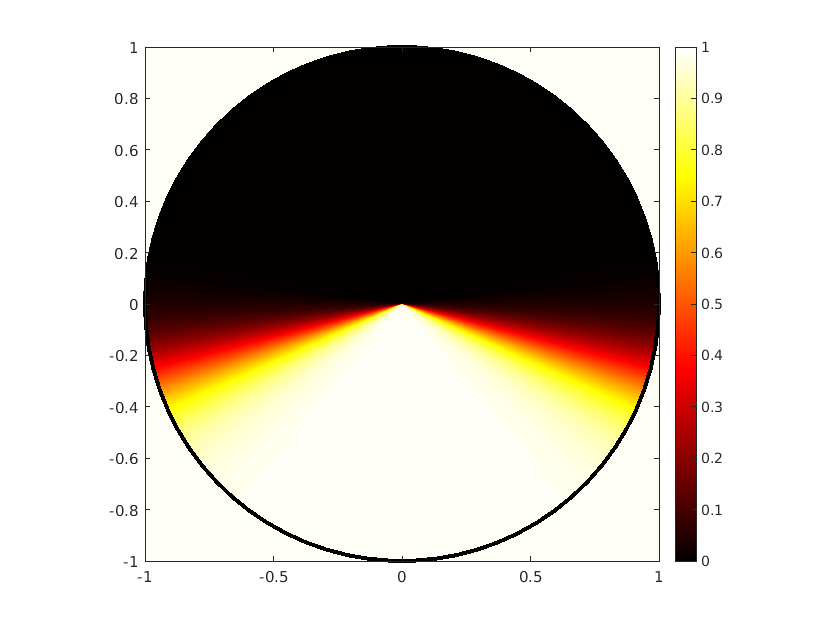
\includegraphics[width=0.6\columnwidth,trim=125px 0px 125px 0px,clip]{images/leaderweight_logistic.png}
        \hspace*{0.15\columnwidth}
    }
    \par
    \subfloat[Velocity average sensitivity (logistic from equation \ref{eqn:individualVelocityWeighting}): $1/(1+\exp(-w_{va}\hat{\bm{r}}_{ij}(t)\cdot\hat{\bm{v}}_i(t)+w_{vb}))$\\ with $w_{va} = 6.79$, $w_{vb} = 2.20$]{
        \hspace*{0.15\columnwidth}
        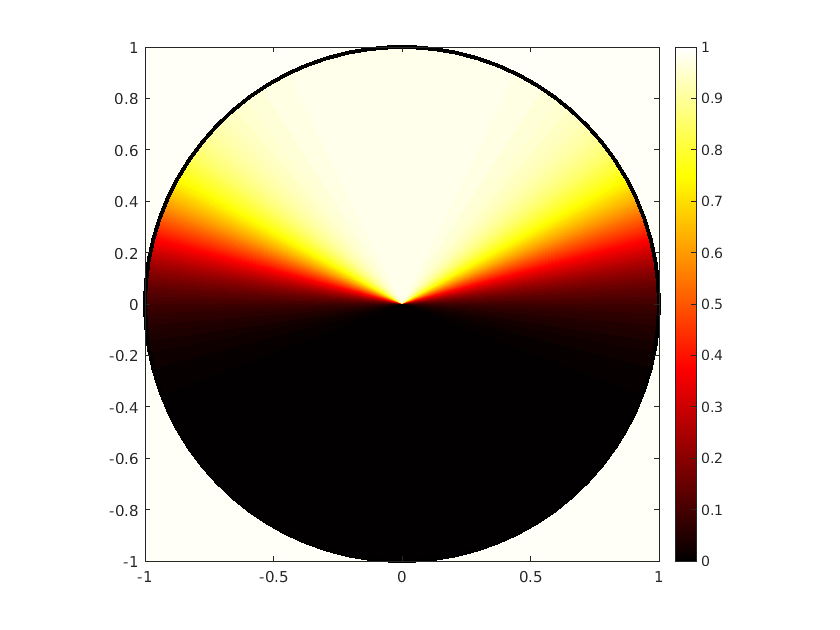
\includegraphics[width=0.6\columnwidth,trim=125px 0px 125px 0px,clip]{images/vweight_logistic.png}
        \hspace*{0.15\columnwidth}
    }
    \par
    \subfloat[Position average sensitivity (logistic from equation \ref{eqn:individualPositionWeighting}): $1/(1+\exp(-w_{xa}\hat{\bm{r}}_{ij}(t)\cdot\hat{\bm{v}}_i(t)+w_{xb}))$\\ with $w_{xa} = 1.35$, $w_{xb} = -0.85$]{
        \hspace*{0.15\columnwidth}
        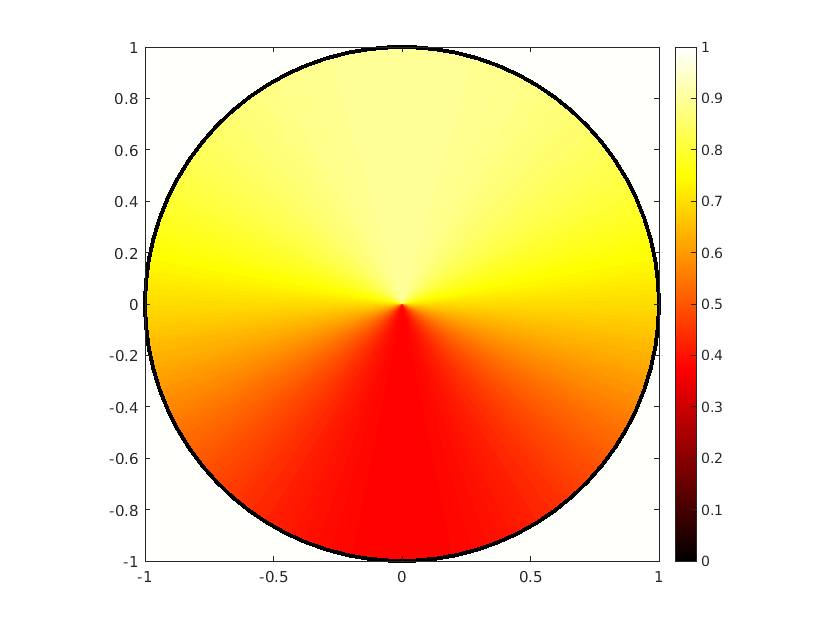
\includegraphics[width=0.6\columnwidth,trim=125px 0px 125px 0px,clip]{images/cmweight_logistic.png}
        \hspace*{0.15\columnwidth}
    }
    \caption{Sensitivity of entities to neighbor parameters.}
    \label{fig:logisticSensitivities}
\end{figure}

The logistic functions that appear in equations \ref{eqn:leaderRegionContribution}, \ref{eqn:individualVelocityWeighting}, and \ref{eqn:individualPositionWeighting} give each entity anisotropic sensitivity to the position and velocity of its neighbors.
Fig. \ref{fig:logisticSensitivities} plots this senstivity, assuming the forward direction of travel of the entity is upwards, with white corresponding to a high sensitivity (weight 1) and black low sensitivity (weight 0).
The leader factor sensitivity is slightly different: unlike the other two which have maximal sensitivity to the front of the entity, the leader factor is most sensitive to entities behind it.

\section{Results and Discussion}

\begin{figure*}[htbp]
    \centering
    \subfloat[]{
        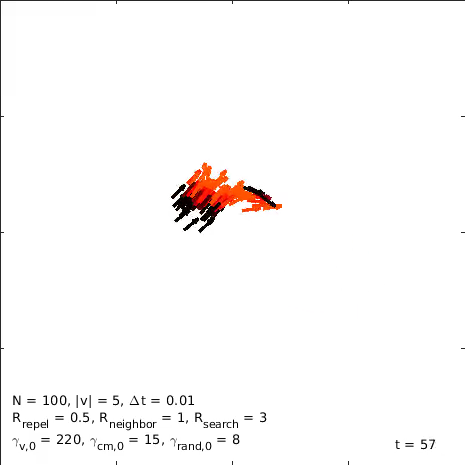
\includegraphics[width=0.6\columnwidth,trim=5px 5px 5px 130px,clip]{images/vlcsnap-2022-05-09-21h00m12s165.png}
        \label{fig:torus1}
    }
    \quad
    \subfloat[]{
        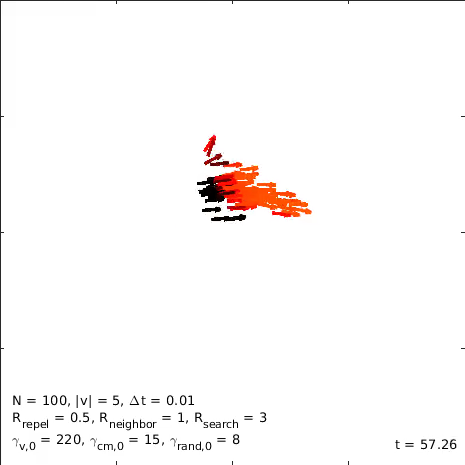
\includegraphics[width=0.6\columnwidth,trim=5px 5px 5px 130px,clip]{images/vlcsnap-2022-05-09-21h00m18s947.png}
        \label{fig:torus2}
    }
    \quad
    \subfloat[]{
        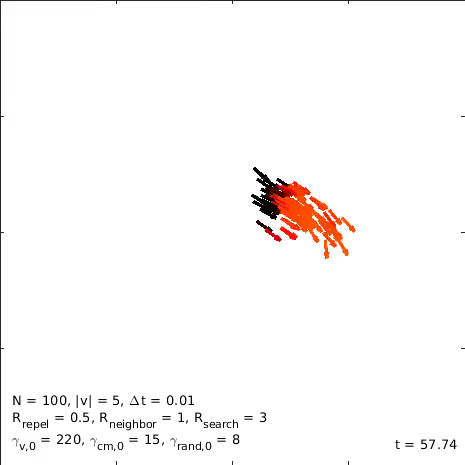
\includegraphics[width=0.6\columnwidth,trim=5px 5px 5px 130px,clip]{images/vlcsnap-2022-05-09-21h00m22s857.png}
        \label{fig:torus3}
    }
    \par
    \subfloat[]{
        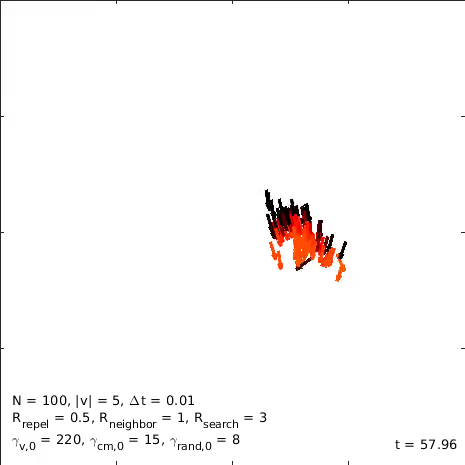
\includegraphics[width=0.6\columnwidth,trim=5px 5px 5px 130px,clip]{images/vlcsnap-2022-05-09-21h00m26s463.png}
        \label{fig:torus4}
    }
    \quad
    \subfloat[]{
        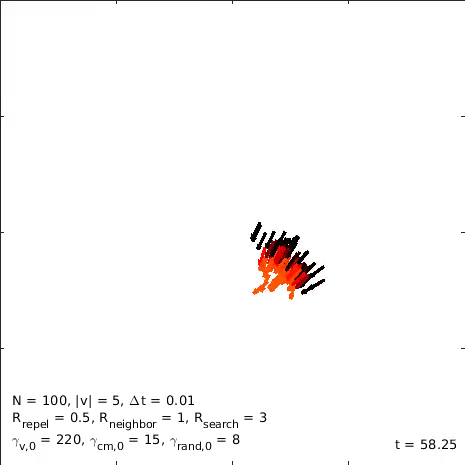
\includegraphics[width=0.6\columnwidth,trim=5px 5px 5px 130px,clip]{images/vlcsnap-2022-05-09-21h00m29s530.png}
        \label{fig:torus5}
    }
    \quad
    \subfloat[]{
        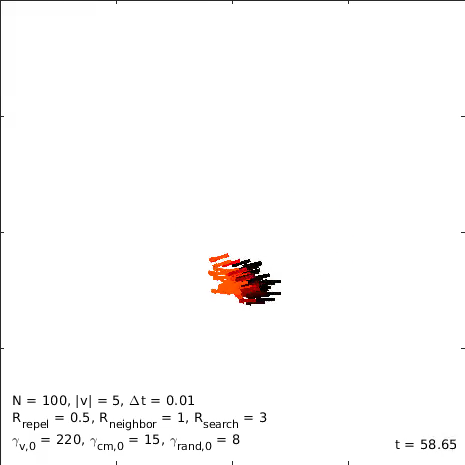
\includegraphics[width=0.6\columnwidth,trim=5px 5px 5px 130px,clip]{images/vlcsnap-2022-05-09-21h00m32s830.png}
        \label{fig:torus6}
    }
    \par
    \subfloat[]{
        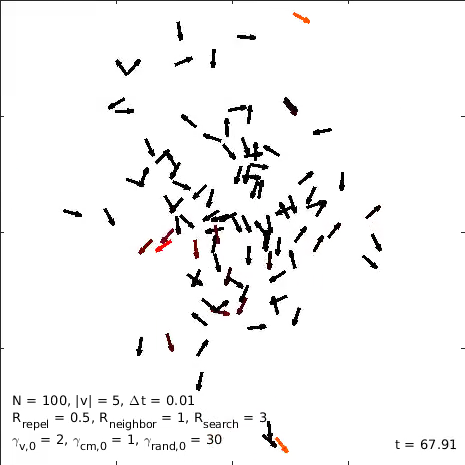
\includegraphics[width=0.6\columnwidth,trim=5px 5px 5px 5px,clip]{images/vlcsnap-2022-05-09-21h01m15s943.png}
        \label{fig:scatteredmotion}
    }
    \quad
    \subfloat[]{
        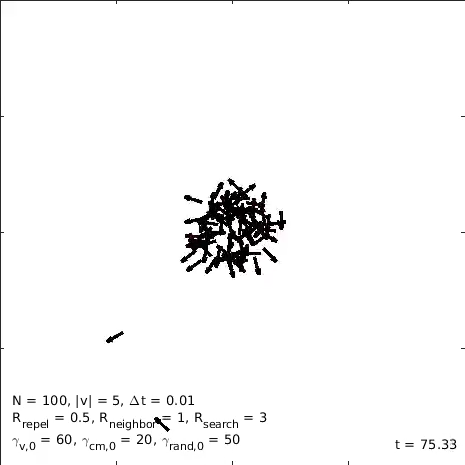
\includegraphics[width=0.6\columnwidth,trim=5px 5px 5px 5px,clip]{images/vlcsnap-2022-05-09-21h01m22s136.png}
        \label{fig:swarming}
    }
    \quad
    \subfloat[]{
        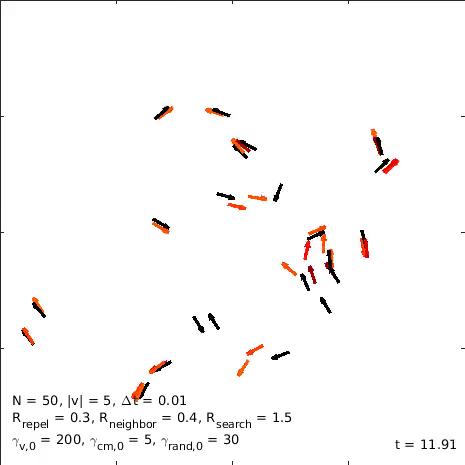
\includegraphics[width=0.6\columnwidth,trim=5px 5px 5px 5px,clip]{images/vlcsnap-2022-05-09-21h22m11s622.png}
        \label{fig:separate}
    }
    \caption{
        Movement patterns observed for various weightings of the driving terms in equation \ref{eqn:newton}.
        Fig. \ref{fig:torus1} - \ref{fig:torus6} show the evolution of a dense pack of entities traveling in a circle, similar to the pattern of a small school of fish.
        Fig. \ref{fig:scatteredmotion} shows very loose, uncorrelated motion, much like the behavior of a colony of ants that has been disturbed.
        In Fig. \ref{fig:swarming}, the entities are swarming like bees when migrating to a new hive.
        Fig. \ref{fig:separate} shows patches of correlated motion in small groups.
        This simulation was done with leader sensitivity parameters $\alpha_\lambda = 20$ and $\beta = 50$;
        random filter time constant $\tau_\xi = 2$;
        parameters for leader factor sensitivity to leader contribution: $w_{\lambda a} = 2.20$ and $w_{\lambda b} = 0$;
        spatial sensitivity parameters for leader contribution $w_{la} = 9.85$ and $w_{lb} = 2.94$;
        spatial sensitivity parameters for velocity and position $w_{va} = 6.79$, $w_{lb} = 2.20$ and $w_{xa} = 1.35$, $w_{xb} = 0$;
        leader sensitivities for velocity, position, and noise forcing terms $\kappa_{\lambda_v} = 0.5$, $\kappa_{\lambda_x} = 0.8$ and $\kappa_{\lambda_{\xi}} = 10$;
        center-of-mass matching attraction zone weight $\kappa_{cm_{\mathcal{R}^a}} = 5$;
        random force term region-density sensitivites $\kappa_{\xi_{\mathcal{R}^o}} = 1$, $\kappa_{\xi_{\mathcal{R}^a}} = 5$
        and repulsion singularity adjustment $\delta = 0.25$.
        The other parameters are listed in each of the plots (and are different between Fig. \ref{fig:torus1} - \ref{fig:torus6}, \ref{fig:scatteredmotion}, \ref{fig:swarming}, and \ref{fig:separate}.
    }
    \label{fig:movement}
\end{figure*}

As can be seen in Fig. \ref{fig:movement}, this description of motion in equation \ref{eqn:newton} is able to produce collective motion in a variety of forms just by changing the parameters $\gamma_{V_{n_0}}$, $\gamma_{cm_0}$, and $\gamma_{\xi_0}$ (assuming the other parameters discussed in the model have been set appropriately --- see the figure caption for a complete list of parameter values).
While relatively complex compared to the simplest models proposed in \cite{Vicsek}, the fact that this model can qualitatively describe the behavior of very different kinds of collective motion is very exciting.

\subsection{Design Choices}
The reason for including velocity orientation matching in all three regions is to avoid sharp snapping behavior when an entity transitions from having no neighbors in its orientation region $\mathcal{R}^o$ to having many neighbors.
This transition can happen very quickly when the entity moves into a densely populated area as directed by the center-of-mass attracting term $\gamma_{cm_0}\mathbf{x}_{cm_i}(t)$ in equation \ref{eqn:newton}.
The design choice is based off of what animals do in real life when rejoining a moving group: they gradually transition from traveling towards the center of the group to matching its speed rather than moving straight to the group and only changing direction when they get there.

Logistic functions were chosen for weighting the forcing term contribution for different velocity-displacement dot products $\theta_{ij}(t)$ because they have a range $(0,1)$ and provide a gradual transition between 0 and 1 (as can be seen in Fig. \ref{fig:logisticSensitivities}).

\subsection{Future Considerations}
Although outside the scope of this project, implementing adaptive partitioning of the coordinate plane with a tree data structure would likely improve the performance of the neighbor search algorithm.
Currently, the neighbor search is the limiting factor when attempting to simulate the behavior of large groups (e.g. $N > 50$).
Improving the grid partitioning would allow for the minimum number of partitions while keeping the number of entities within each partition roughly constant, reducing the time spent searching for neighbors.

\begin{thebibliography}{00}
    \bibitem{Vicsek} T. Vicsek, A. Zafeiris, ``Collective Motion," Physics Reports, vol. 517, pp. 71-140 (2012)
    \bibitem{Couzin} I. D. Couzin, J. Krause, R. James, G. D. Ruxton, N. R. Franks, ``Collective Memory and Spatial Sorting in Animal Groups," J. theor. Biol., vol. 218, pp. 1-11 (2002)
\end{thebibliography}

\end{document}
